% !TEX root = ../thesis.tex
%
\chapter{Pipeline}
\label{sec:pipeline}

\section{Generating detections}
\label{sec:pipeline:eval}
Our desired output of the algorithm is one or are multiple boxes enclosing each a section of the image which is predicted to contain the searched for type of object. The \gls{fcn} returns a score map as output. Each score predicts the probability of this pixel to be of the class we trained for. Therefore we need a method to return high scoring bounding boxes from a probability map. The here employed way of doing this consists of multiple steps:\\
\begin{enumerate}
    \item We penalize (near-) empty regions inside the probability map with a negative distance transform
    \item We generate a set of beforehand defined boxes
    \item For all these boxes we calculate the score density
    \item We apply a low threshold to filter out unnecessary boxes
    \item We apply non maximum suppression to get the top scoring boxes
\end{enumerate}

\subsection{Negative Distance Transform}
\label{sec:pipeline:eval:dt}
\begin{figure}[htb]
    \begin{tabular}{ccc}
        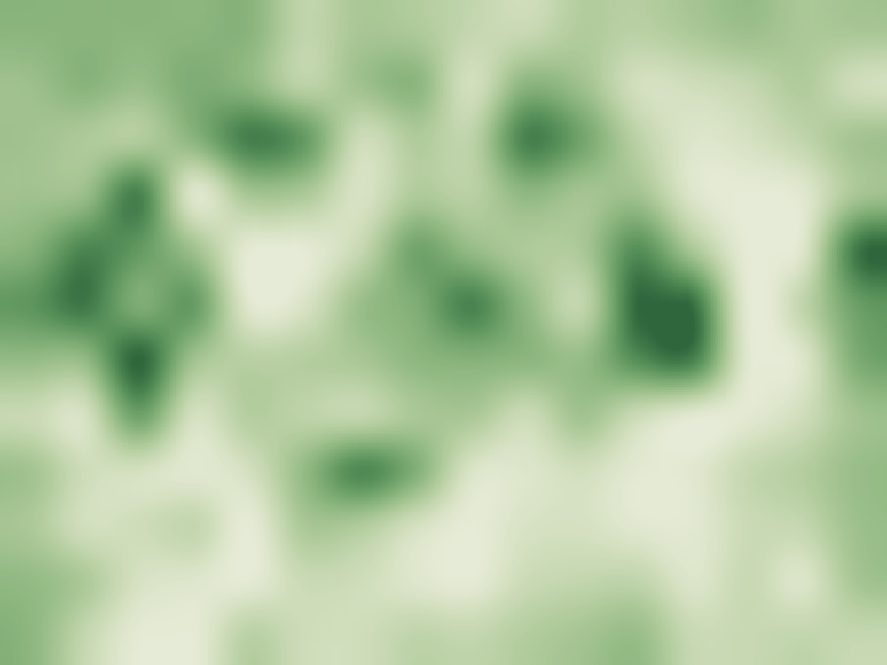
\includegraphics[width=45mm]{figures/build/distance_transform_hm} &
        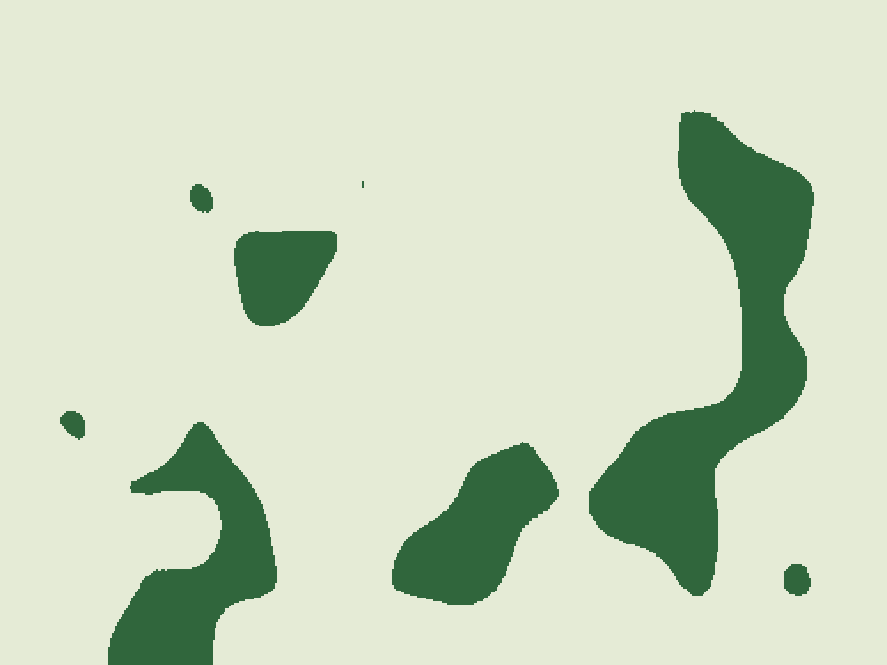
\includegraphics[width=45mm]{figures/build/distance_transform_thres} &
        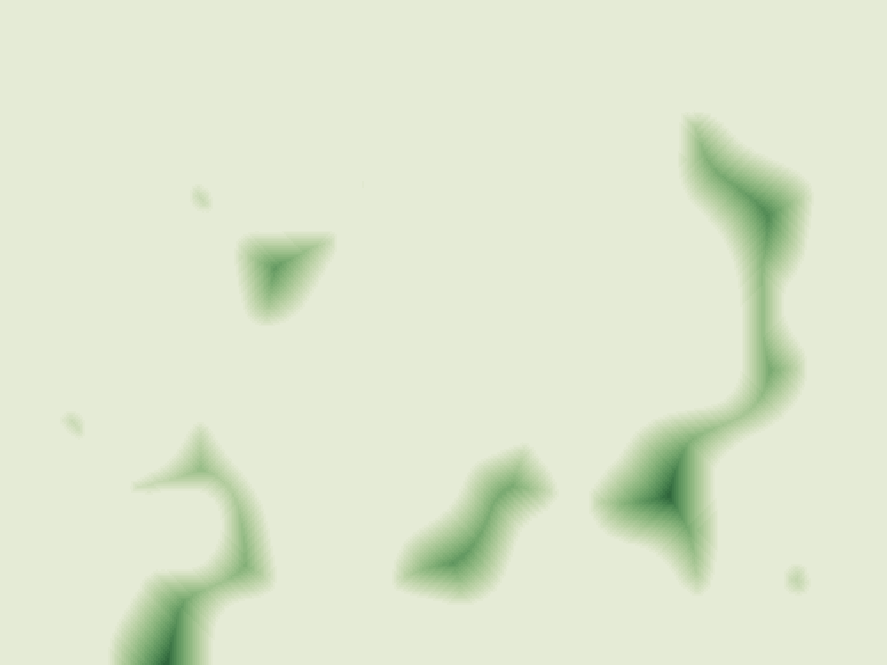
\includegraphics[width=45mm]{figures/build/distance_transform_negative} \\[6pt]
        (a) A probability map & (b) Thresholded map & (c) Distance transform
    \end{tabular}
	\caption{Computing the negative distance transform from an probability map}
    \label{fig:distance_transform}
\end{figure}
A lot of images produce probability maps that are sparsely filled. We want to penalize these regions. Positive regions receive a positive score from the network while not-positive regions are at-most zero. Here we introduce a distance transform to score regions of near-zero values \fref{fig:distance_transform}. First we threshold the score map with a near-zero value to set all values that can safely assumed to be negatives to zero. Second we apply a distance transform to the zero part of the binary image. A distance transform labels each zero pixel of an image with its distance to the nearest one valued pixel. The distances are valued with some metric like the Euclidean distance or the $L_1$ distance. As the specific metric is not important for our vague penalizer and as we aim for good time performance we use the $L_\infty$ distance also known as the chessboard distance. The transformed image is normalized and substracted from the original probability map.

\subsection{Calculating the score densities}
\label{sec:pipeline:eval:density}
For each forwarded image we generate a set of boxes to calculate the score densities for. At three scales we take boxes of the same aspect ratio as the input image and calculate the slices that would be the result of sliding the window over the image. Also we save the area of all rectangles.\\
Density is calculated by summing up all the probabilities from the score map inside the current window and dividing this sum by the area of the window. To achieve that as efficiently as possible we use the integral image of our score map. By summing up all values from the top-left corner to the bottom-right corner of an image we get its integral. A value of the integral then is the sum of all values inside the rectangle of this point and the top-left corner:
\begin{equation}
    I_{int}(x, y) = \sum_{\substack{x' \le x\\ y' \le y}} I(x', y')
\end{equation}
The sum inside any rectangle can then computed efficiently with:
\begin{equation}
    \sum_{\substack{x_0 < x \le x_1\\ y_0 < y \le y_1}} = I_{int}(x_1, y_1) + I_{int}(x_0, y_0) - I_{int}(x_1, y_0) - I_{int}(x_0, y_1)
\end{equation}

\subsection{Non maximum suppression}
\label{sec:pipeline:eval:nms}
Depending on the number of scales we generate hundreds or even thousands of boxes per image. We want to eliminate boxes that are overlapping with another box that has a higher density. Firstly we drop the worst boxes with a low set threshold. To the remaining boxes we apply non maximum suppression as described by \citet{felzenszwalb_discriminatively_2008}. In the non maximum suppression we first sort all boxes by their descending scores which in our case are the probability densities. We mark the strongest box as picked. Then we calculate the area overlap between the new picked box and all remaining boxes. All boxes with an overlap in area of 0.5 or more are dropped. We pick the next strongest score of the remaining set and continue this process until all boxes are either dropped or picked. The strongest not-overlapping boxes remain picked and are returned.
